\section{Data Analysis and Results}
\label{Sec:DataAnalysisAndResults}
In the following section, the hand-washing trials, the SRS survey, entrance survey, and post-interventions survey, and the parent interviews were analyzed qualitatively, and the annotated video data of the hand-washing trials was analyzed quantitatively.

\subsection{Participants Recruited}
Due to limitation of time, we were only able to recruit one subject.  Our participant is a thirteen year old male child of Asian ethnicity.  He was accompanied to the trials by his mother, who was the one that answered all surveys.

\subsubsection{Entrance and SRS Survey Results}
The following background of the child was reported by the entrance and SRS surveys.  The purpose of this section is to familiarize the reader with our participant and understand better the context that our study results situate in.

\paragraph{Child's Demographics and Inclusion Criteria Fit}
The parent reported that the child has been clinically diagnosed with Autism spectrum disorder.  We also conducted the Social Responsiveness Scale Survey, and the child obtained a T-score of 79, passing the minimum score for severe ASD.  Through the Entrance Survey, we learned that the child has difficulty independently completing self-care activities (a 2 on a scale of 1 (not independent at all) to 5 (completely independent)), and this includes hand-washing (also a 2 on the same scale).  We also learned that the child is able to but not good at verbal communication (a 3 on a scale of 1 (very not well) to 5 (very well)).  Specifically, the child can only speak one or two words at a time to express what he wants, uses iPad for communication, and often just murmurs illegibly.  However, the child has the ability to follow simple, one-step verbal instructions (a 4 on a scale of 1 (very not well) to 5 (very well)).  Lastly, the child does not exhibit severely aggressive behavior (a 1 from a scale of 1 (never) to 5 (often)).  The above shows that the child fits our inclusion criteria.

\paragraph{Child's Experience with Technologies}
The child is more of a visual learner.  He uses a computer at home, and likes to use it very much.  He also likes to use other technologies (e.g. iPhone, iPad), and likes to watch movies and TV.  He does not have a robot toy to play with at home or at school, so the parent does not know how much he likes to play with robot toys.  The parent never used technologies to help the child with self-care activities except using pictures to teach step by step hand-washing.

\paragraph{Child's Personal Preferences}
The child is sensitive to sound.  He likes Disney cartoon music, and likes to watch his favorite cartoon scenes repeatedly on the iPad.  To reward the child after a good behavior, the parent suggested the following rewards: give extra time to play on iPad, give him praises (e.g. good job), give children books to read and animal dinosaurs to play with, give the parent's iPhone since the child's favorite musics are on there.

\paragraph{Child's Abilities on Hand-washing and on Other ADLs}
The parent agrees that the child usually gets distracted when performing hand-washing.  To assist him, the parent mainly reminds him to put soap, rinse properly, and dry properly with towel.  He needs more prompting in these areas since he always washes in a hurry.

Other everyday activities the child needs help with include:  tooth brushing -- 2 hours/week; bathing -- 4.5 hours/week; dressing -- usually just hand the clothes to him, he knows how to put them on, but needs reminders of the order of the clothing, 7 hours/week.

\paragraph{Parent's Expectation and Concerns}
The parent expected the robot to be helpful in reminding the child to put soap, rinse and dry more, similar to the role of M.  Some concerns the parent has include: the child may be wondering why does he need to wash hands so many times repeatedly; the child performs well in his comfort zone with the same environment, so it takes a while for the child to get used to the lab environment.

\subsection{Case and Samples Selected}
Our participant fitted the inclusion criteria as a user with typical use case for the robot.  It was noted that the typical use cases for the robot may be several, depending on the kinds of helps the user needs.  From the background report above, we understood that the child mainly needs help initiating the hand-washing activity, and guidances during certain steps (i.e. the get soap, rinse, and dry steps), but the child does not need much prompts for demonstrating the actions of each step.  This tendency of the child was verified during the trials, and we attempted to answer the question ``how best to prompt the child'' given this tendency (e.g. Should we prompt only the steps the child needs help, or prompt every step to create consistency?  Should we still demonstrate actions for the prompted steps or skip the MoDemo part of the prompt entirely?)  These will be answered in our discussions.

As part of the effort for employing maximum variation sampling method, we had different phases of trials having a variation of the prompting agents involved.  In addition, for the phase with parent and robot joint prompting (i.e. Phase C), the researcher and the parent discussed before each trial how much the parent involved in helping the child for that trial, with the goal to fade out the involvement to minimal by the end of Phase C, while maintaining a high level of child's compliance to robot prompts.  To describe specifically, across the four phases, there were five levels of involvement employed:
\begin{itemize}
	\item \textbf{Level 0}: the parent is outside of the room out of the child's view, only comes into the washroom to prompt when the child is not following the robot (this behavior is similar to that during Phase B)
	\item \textbf{Level 1}: the parent stands beside the child in the washroom, and mainly uses gestures to prompt the child to follow the robot and to demonstrate the step's motions after robot prompts
	\item \textbf{Level 2}: the parent stands beside the child in the washroom, and uses both verbals and gestures to prompt the child about each hand-washing steps, in competition to the robot prompts
	\item \textbf{Level 3}: the parent stands behind the child, and physically guide the child to follow the robot prompts
	\item \textbf{Level 4}: the parent stands beside the child, and prompts as the parent sees fit each hand-washing steps, with no robot present
\end{itemize}
The Parent Involvement Level is plotted in Figure \ref{fig:6ParentInvolvement}.  We see that, in Phase C, the parent mainly alternated between trial segments of level 1 and level 3 to train the child to follow the robot, while mixing single trials of level 0 to monitor the child's progress when left with robot alone.
\begin{figure} [h]
	\centering
	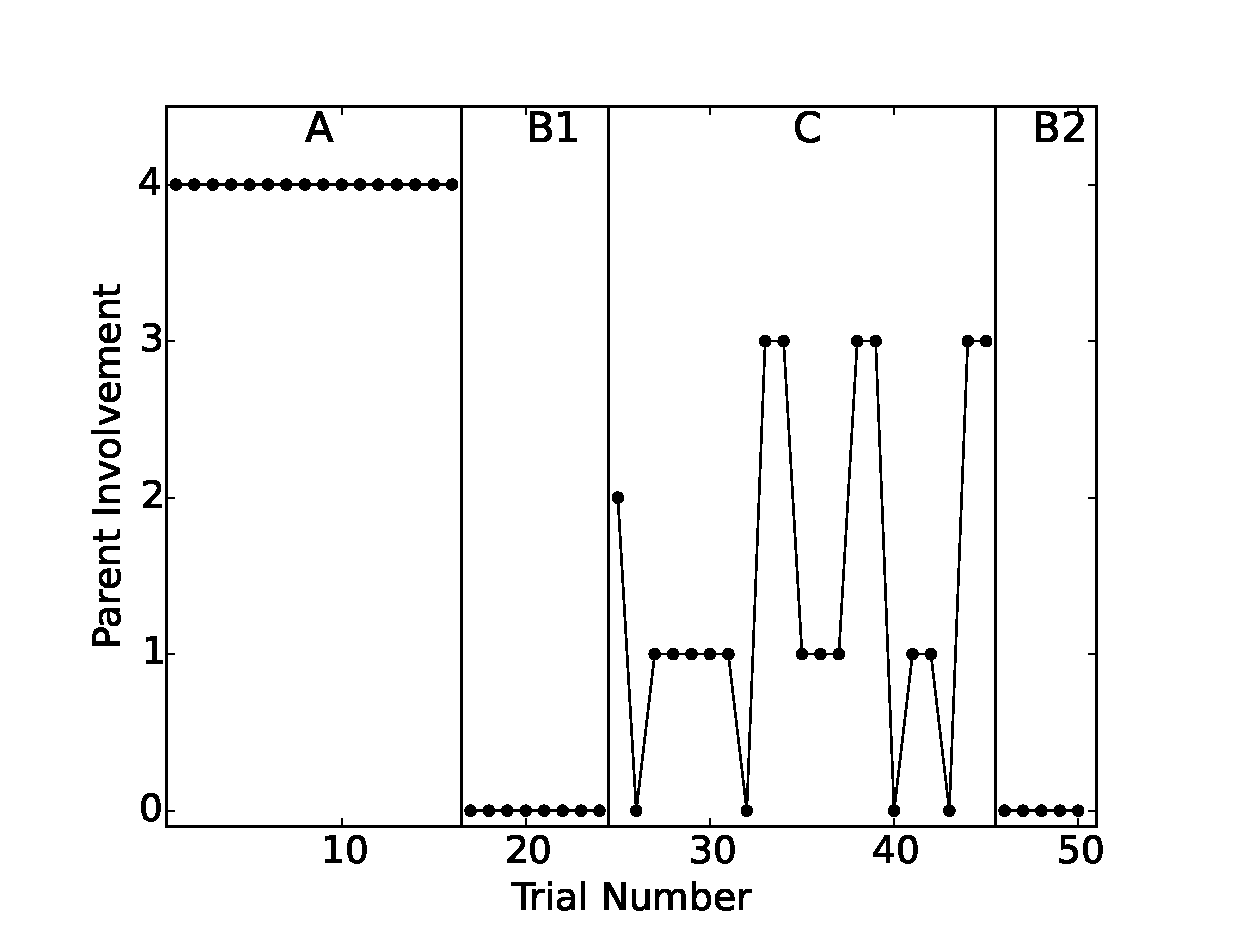
\includegraphics[width=0.6\textwidth]{./img/data_analysis/6ParentInvolvement.eps}
	\caption{Parent Involvement}
	\label{fig:6ParentInvolvement}
\end{figure}

As part of the study protocol, the parent was allowed to physically help the child through a step if other methods of prompting failed.  This intervention from the parent involved either the parent guiding the arm of the child during step execution or doing the step fully for the child.  Specifically, the number of prompts that the parent intervened in this manner were counted and plotted, shown in Figure \ref{fig:7NumberofParentPrompts-PhysInterv}.  We see the parent minimally physically intervened during Phase A and Bs but intervened much more during Phase C (the joint prompting training phase).
\begin{figure} [h]
	\centering
	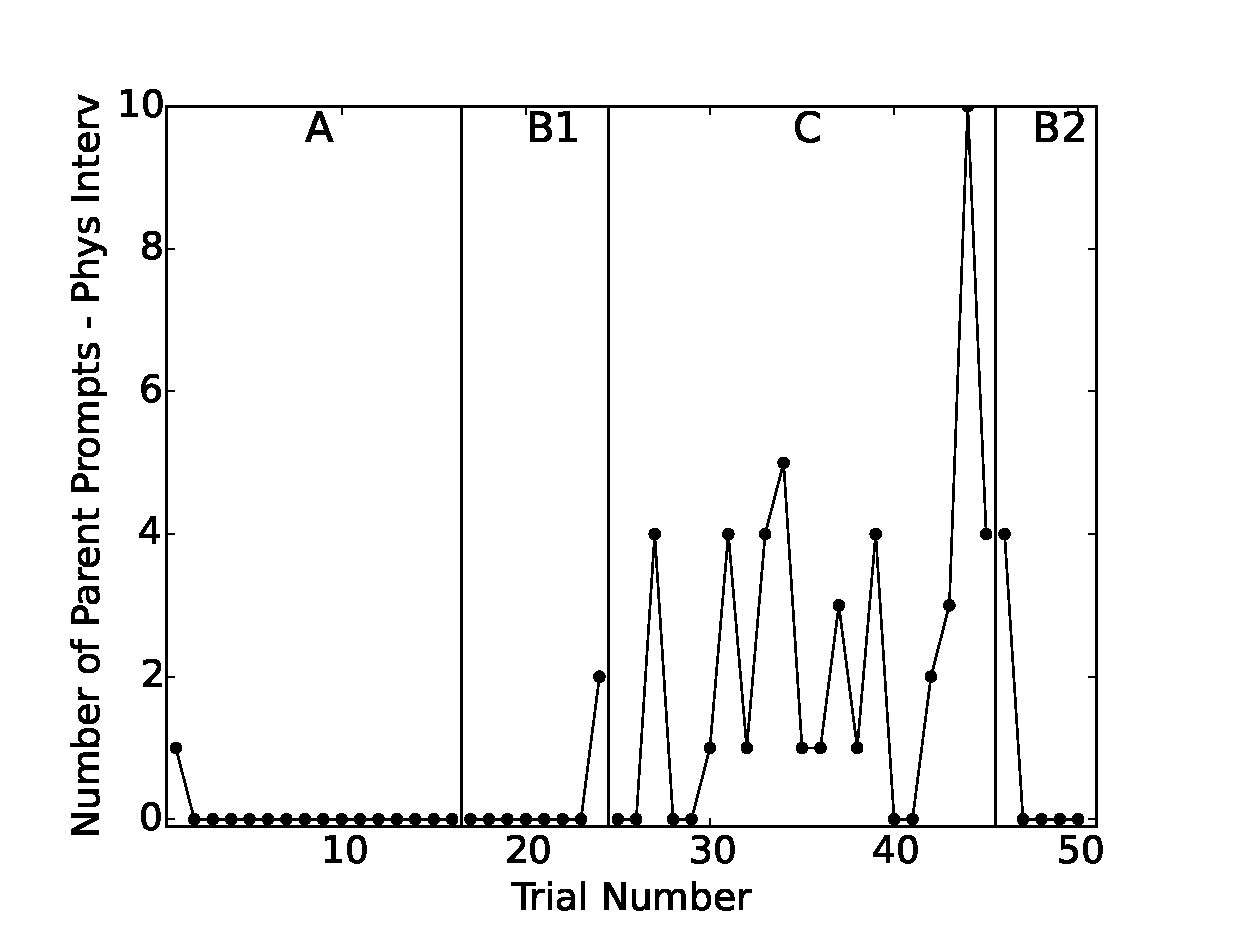
\includegraphics[width=0.6\textwidth]{./img/data_analysis/7NumberofParentPrompts-PhysInterv.eps}
	\caption{Number of Parent Prompts - Physical Intervention}
	\label{fig:7NumberofParentPrompts-PhysInterv}
\end{figure}


\subsection{Quantitative Analysis and Results - Preliminary}
\label{sec:QuantitativeData_results}
The annotated video data are analyzed quantitatively by calculating the measures defined in Section \ref{sec:measures} to investigate how well can the child wash hands with the help of the parent and the robot and how well does the child respond to the prompts.

\subsubsection{Quantitative Analysis Method}
A script written by the researcher in Python 2.7 with NumPy scientific computing package was used to calculate the measures from the CSV files generated from video annotations.  Matplotlib package was used for plotting.  We compared each measure across the phases by calculating the median of all the trials in each phase.  The median was chosen for robustness against outliers.  No further statistical analyses were employed because of the small sample size involved.

\subsubsection{Task Completion}
The ``Number of Steps Completed'' by the child, for both steps completed independently and steps helped by a prompting agent, are plotted in Figure \ref{fig:0NumberofStepsCompleted-Overall}.  The figure shows that Phase A has a median of 6 steps completed, while the rest of the phases have a median of 5 steps being completed.  The missing step in all phases is the wet hands step.  The parent in Phase A never prompted for the wet hands steps, and thus it was never completed in Phase A.  This was because the child was used to getting soap first with dry hands before turning on the water for rinsing.  The researcher, upon observing this, decided to skip prompting for the wet hands step as well for the subsequent phases, and thus all phases are missing the completion of the wet hands step.  The missing step specifically for Phase Bs and C is the scrub hands step.
\begin{figure} [h]
	\centering
	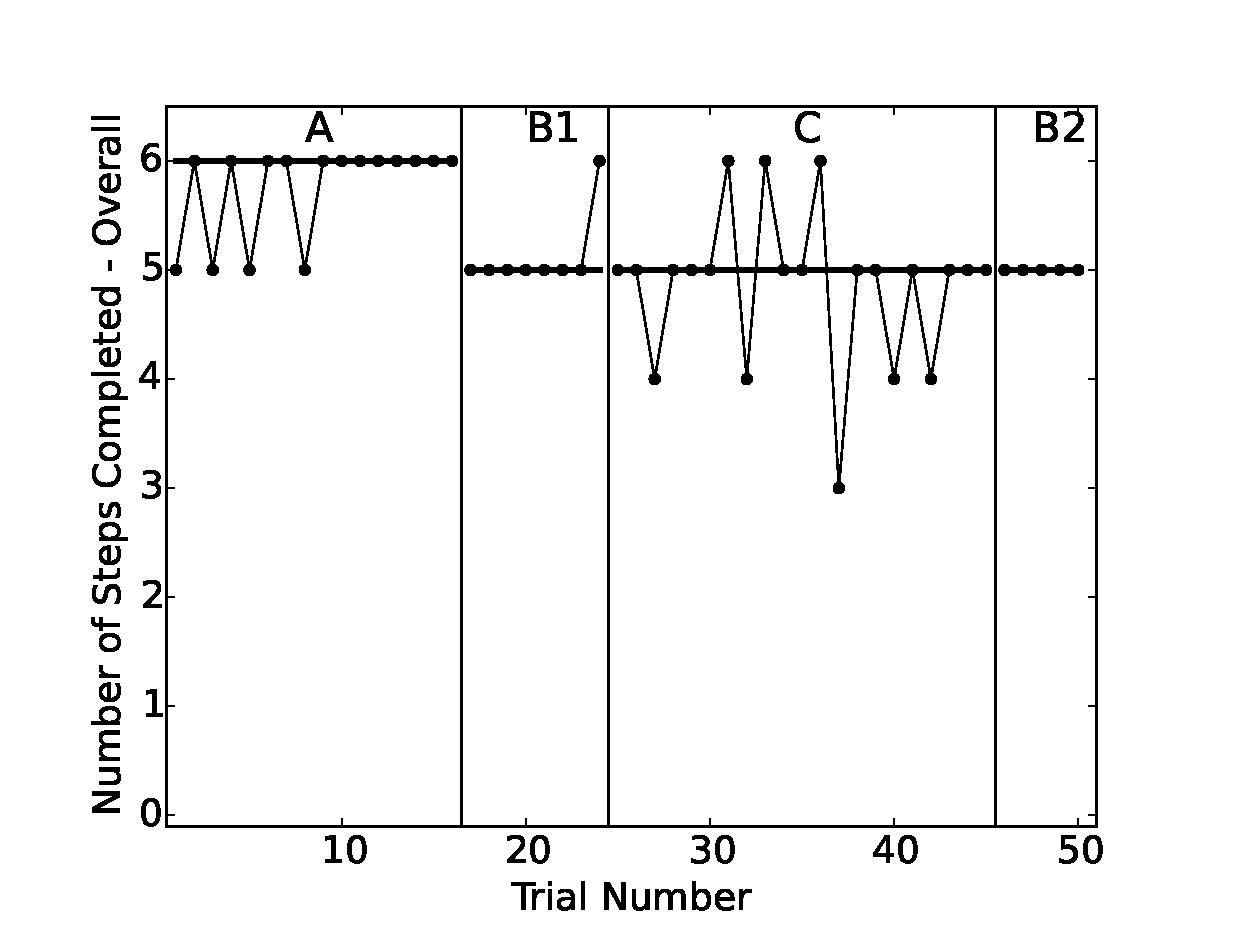
\includegraphics[width=0.6\textwidth]{./img/data_analysis/0NumberofStepsCompleted-Overall.eps}
	\caption{Number of Steps Completed - Overall}
	\label{fig:0NumberofStepsCompleted-Overall}
\end{figure}

In Phase A, where the parent would prompt the scrub step right after the child finished getting soap as well as demonstrating the motion of scrub in the air.  The child was looking at the parent's MoDemo prompts and was following the motions himself.  In the subsequent phases, when the robot prompted the scrub step with MoDemo, the child did not follow, and would start rinsing instead.  The researcher decided to skip robot prompting for the scrub hands step, and focused on the rinse step prompts instead.  In whole, although the expectation of which steps to be completed shifted from six steps in Phase A into five steps in Phase Bs and C, the child mostly completed the steps up to expectations in all trials.  This was a result of the child's own independent ability to complete hand-washing, the help of the robot prompts, the help of the parent's prompts, and at times the result of the parent completing the step for the child.



\subsubsection{Child's Response to Prompts}
In order to break down how much of the task completion was due to the prompts from the parent and the robot, we measured the ``Complied Prompt Rate'' and the ``Ignored Prompt Rate''.  To define these two measures, we observe that for each prompt, there are three components: the step the child was executing before the prompt, the step being prompted, and the step the child executes after the prompt.  Also, the child could be executing the correct step being prompted, could be executing the wrong step, or could be idling without executing any step.

Compliance to a prompt, then, is defined as when the child was executing the wrong step or was idling before prompt, and is executing the right step after the prompt.  In addition, when the step is an extended step (e.g. scrub, rinse, dry), which requires multiple prompts, compliance can also be seen when the child was executing the correct step both prior to and after the prompt.  The ``Complied Prompt Rate'' is plotted in Figure \ref{fig:4ComplianceRate-Overall}, and the median for Phase A is 87\%, for Phase B1 is 33\%, for Phase C is 77\%, and for Phase B2 is 80\%.

The child is said to ignore the prompts when the child does not change the step before and after the prompt.  Specifically, this happened if the child was executing the wrong step before prompt and remains executing that same wrong step after the prompt, or when the child was idling before prompt and remains idling after prompt, or when the child executes the correct non-extended step before and after the prompt (this usually happened because the robot delivered the prompt too late although the child knew what to do or when the parent prompted for the child to stop the getting soap step but the child did not comply).  The ``Ignored Prompt Rate'' is plotted in Figure \ref{fig:1NotAffectedByPromptRate-Overall}, and the median for Phase A is 10\%, for Phase B1 is 33\%, for Phase C is 8\%, for Phase B2 is 13\%.
\begin{figure} [h]
	\centering
	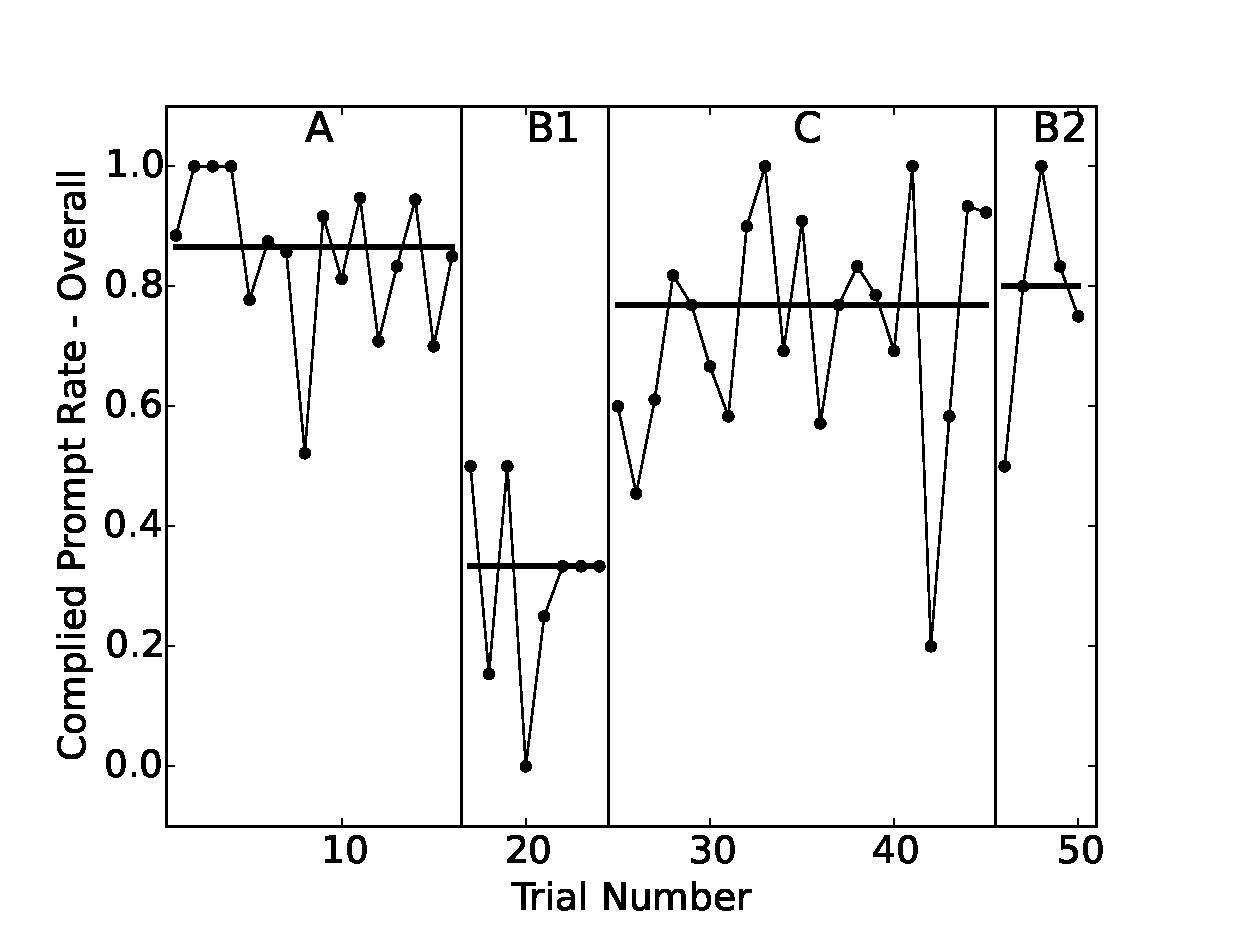
\includegraphics[width=0.6\textwidth]{./img/data_analysis/4CompliedPromptRate-Overall.eps}
	\caption{Complied Prompt Rate - Overall}
	\label{fig:4CompliedPromptRate-Overall}
\end{figure}
\begin{figure} [h]
	\centering
	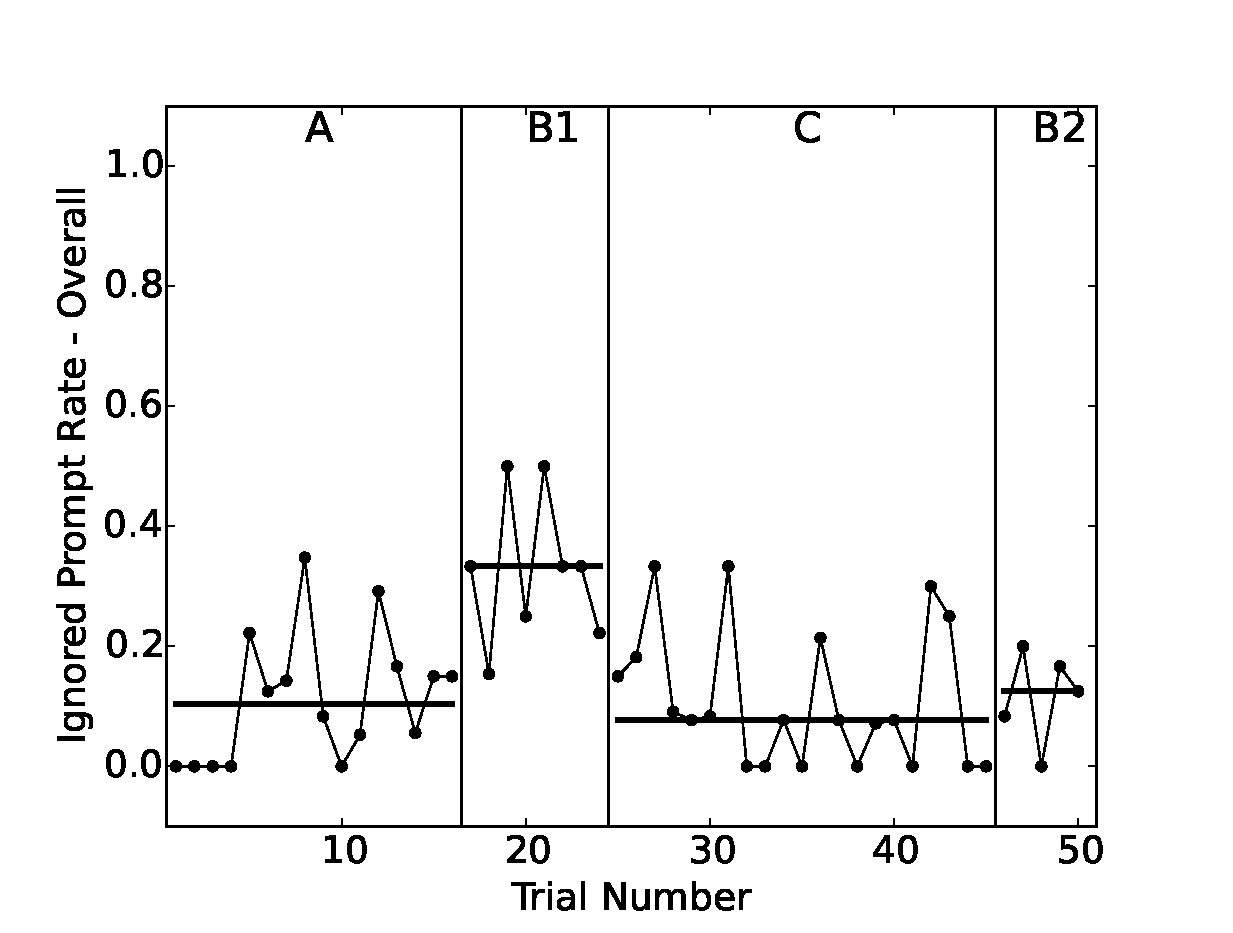
\includegraphics[width=0.6\textwidth]{./img/data_analysis/1IgnoredPromptRate-Overall.eps}
	\caption{Ignored Prompt Rate - Overall}
	\label{fig:1IgnoredPromptRate-Overall}
\end{figure}


\subsection{Qualitative Analysis and Results}
\label{sec:QualitativeData_results}
The preliminary quantitative analysis above showed that the child had low compliance to robot prompts in Phase B1 compared to parent prompts in Phase A, and experienced an increase in compliance in Phase B2, probably due to the trainings in Phase C.  We now use qualitative analysis to report what happened in a more descriptive manner, and attempt to answer what contributed to the low robot prompt compliance and its improvement.

We conducted 16 trials for Phase A, 8 trials for Phase B1, 21 trials for Phase C, and 5 trials for Phase B2.  For analysis, we first compared and contrasted between parent prompting and robot prompting on how the prompts were delivered and how well did the child receive them.  Then we examined the factors contributing to the child's difference of reception of robot prompts and the parent prompts.  Lastly, we explored changes to the robot and the study that did or would possibly improve robot prompt reception from the child.

\subsubsection{Qualitative Analysis Method}
The sources of data collected for qualitative data analysis included child hand-washing trials videos, between trials parent researcher interview transcriptions, and the post-intervention survey.

The hand-washing trials videos were reviewed by the researcher while making field notes on what were the patterns of the prompting agents, and the behavior patterns of the child, including both the child's independent actions during hand-washing as well as the child's reactive actions to prompts.  These field notes, together with the parent interviews, were analyzed using the ``constant comparative method'' to distill common categories or themes that cut across all trials.  In concise words, the ``constant comparative method'', as described by Merriam, is an analysis method commonly used in qualitative research that involves comparing ``one unit of information with the next in looking for recurring regularities in the data'' \cite{merriam2014qualitative}.  Categories are formed that the data relevant to the research questions fit into.  As we go through more units of information, these categories may be subdivided or subsumed under more abstract categories as we ``begin to discriminate more clearly between the criteria for allocating data to one category or another''.  As a side note, this process focuses on describing the data in a concise and logical way rather than on evaluating hypotheses.

Lastly, the parent's post intervention survey was also reported.  In addition, the researcher would self reflect on how to improve the robot, the prompting protocol, and the research study and give inputs as the person who operated the robot and conducted the study.

\subsubsection{Parent Prompts - Phase A}
During Phase A, where the parent alone prompted the child through hand-washing steps, the parent was not instructed on what or how to prompt by the researcher.  The only input given to the parent during this phase was to get the child to rinse more and dry more.  The parent had no prior knowledge of how the robot prompts were going to be like either.  Thus, the way the parent prompted was very similar to how she would have prompted at home in everyday settings, and one she probably found effective to her son.

The sequence of hand-washing steps the parent prompted was in the following order: get soap, lather (synonym to scrub), turn on water, rinse, turn off water, dry.  This order is one of the many logical orders of hand washing, since, for example, one could alternatively choose to turn on water before lather so one could lather in the running water, or even to turn on water before getting soap, so one's hand is wet when lathering.  However, the parent chose to get soap and lather first before turning on water, probably because of her and the child's habits, and she had not changed this sequence order through out the trials in Phase A.  Although, an interesting thing to note is, whenever the parent did not prompt for lather right after get soap and leave the child to decide which steps to do, the child would always turn on the water first after getting soap and lather in water.

The parent used verbal prompts as the major prompting modality, although for some steps, she also prompted using gestures such as pointing and motion demonstration.  The parent's prompting patterns most common for each step are summarized in Table \ref{tab:ParentPrompts}.  In the table, ``MoDemo'' refers to motion demonstration gestures (e.g. rubbing hands together for lather step and flipping and turning hands in the air for dry step).  ``Point'' refers to pointing to the object of interaction (e.g. the water during rinse step).

\begin{table}[H]
	\centering
	\begin{tabular}{ | l | l | l | }
		\hline
		\textbf{Step}	&	\textbf{Verbal Prompt} & \textbf{Gesture Prompt}	\\	\hline	\hline
		
		Get soap	&	Get some soap; Soap;	&	- 	\\	\hline
		Stop soap	&	Just one; That's it; Enough; That's too much;	&	-	\\ \hline
		Lather	&	Lather your hands; Lather; Soap;	& MoDemo	\\	\hline
		Turn on water	&	Turn on the water;	&	-	\\	\hline
		Rinse	&	Rinse more; Water; More water; Wash hands; More;	&	MoDemo; Point	\\	\hline
		Turn off water	&	Turn off the water;	&	-	\\	\hline
		Dry	&	Dry; More Dry; Towel; Dry your hands; More;	&	MoDemo	\\	\hline
		
	\end{tabular}
	\caption{Parent Prompts}
	\label{tab:ParentPrompts}
\end{table}

For the lather, rinse, and dry steps, they are not single action steps, but need continuous motions.  For these steps, the parent would repeatedly deliver verbal prompts of the same step every two seconds or so, until the parent was satisfied with the step's duration.  Variations of the step's verbal prompt were often used (e.g. shortening ``dry your hands'' to ``dry'', or add the word ``more'' or simply using ``more'' for verbal prompts).  The variations can be seen in Table \ref{tab:ParentPrompts}.  Most often for the lather step, and sometimes for the rinse and dry steps, the parent also delivered continuous motion demonstration, and would verbally prompt ``like this'' for the child to follow.  Note that the parent used ``soap'' for verbal prompt of both get soap step and lather step, but the child understood what to do since the parent always delivered motion demonstrations for the lather step.

The timing of prompt deliveries can be categorized as the following:
\begin{itemize}
	\item \textbf{Proactive Prompt}: prompting a new step before the child finishes current step
	\item \textbf{Corrective Prompt}: prompting the same step when the child is doing or is attempting to do a wrong step
	\item \textbf{Reactive Prompt}: prompting when the child is waiting for prompts
	\item \textbf{No Prompt}: letting the child do what he wants without objections
\end{itemize}
The parent delivered proactive prompts most of the times, prompting the next step right when or before the child finished the current step.  However, sometimes corrective prompts were needed when the child was not complying or executing correctly.  There were also a few times that reactive prompts were needed, for example during rinsing, when the child terminated the step early but was waiting for the parent's permission to go on to the next step.  The parent either told the child to keep doing the current step or acknowledged that the child can proceed to the next step.  The last and the least common scenario was the parent delivering no prompts.  This happened when the parent waited to see if the child knew what to do without being prompted, and the child either executed the correct step for the appropriate duration, needing no prompts, or executed incorrectly or for too short or too long of a duration, but the parent let it go without correction.

In addition to the step prompts, the parent also delivered verbal rewards, but usually only at the very end of each hand-washing trial when the child is all done, saying ``good job''.  Also, during the hand-washing, the parent's gaze was mainly focusing on the object being prompted, and very little eye contacts between the parent and the child were seen.  However, during the verbal reward after the child is all done, the parent would often initiate eye contacts.

The child was generally good in complying to the parent's prompts, although at times noncompliance still occurred.  Systematically, the child's compliance can be categorized into the following four scenarios:
\begin{enumerate}
	\item Waiting to be prompted before executing a step
	\item Executing a step as prompted
	\item Keep executing a step until prompted otherwise or verbally awarded
	\item Terminating a step after being prompted for another step
\end{enumerate}
Note that we use the term ``compliance'' loosely here compared to the ``Complied Prompt Rate'' defined in the quantitative analysis section, since not only do we include child's behavior upon prompted as part of the definition here, we also included the child's behavior prior to prompt and the child's behavior during task execution.  And conversely, noncompliance are any scenarios outside of the compliance scenarios.  The five common noncompliance scenarios the exhibited include:
\label{List:NoncopmlianceBehaviors}
\begin{enumerate}
	\item Executing a step before prompted
	\item Executing the wrong step after prompted
	\item Idling after prompted
	\item Terminating a correct step before prompted for another step or verbally awarded
	\item Not terminating a correct step after prompted for another step
\end{enumerate}

Specifically, the child was able to wash hands well under the parent's prompting.  The child would usually start the get soap step first, and he would start the step by himself if the parent did not proactively prompt it.  There were times, however, when the child pressed the soap spout too many times, and the parent had to prompt him multiple times for him to stop.  The lather step was prompted proactively by the parent with MoDemo gestures, and the child followed it obediently for the whole duration, without terminating the step by himself.  The turn on water step is easy for the child, he would do it by himself right after the get soap step and lather in water if the parent did not prompt proactively, or he would execute the lathering step first if the parent prompted proactively for lathering.  The child would always immediately start rinsing (or lathering in water) by himself after turning on water, without waiting for the rinse prompt.  He could execute the motion of this step well, but the challenge was for him to rinse longer.  After about eight seconds of rinsing in water, he would terminate the step by himself, and wait for the parent to prompt the next step.  If the parent continued to prompt for the same step (i.e. rinse more), he would put his hands in the water for one second and withdrew it and wait for the next prompt.  However, he would not start the turn off water step by himself without getting prompted or approval from the parent.  When the parent prompted for turn off the water, the child had no problem following the prompt and executing it.  In addition, he would always start the drying step by himself immediately after turning off the water.  The drying step was a little challenging for the child in both its motion and duration.  The child's motion was mostly drying the inside of his hands, without turning the towel or hand to dry the outside.  However, the parent only demonstrated the motions occasionally, and the child did not change his drying actions even after observing the MoDemo prompts.  The duration of the drying step was around eight seconds before the child decided to terminate the step by himself.  The parent only proactively prompted to dry more while the child was drying, but did not prompt to object when the child decided to terminate the step by putting down the towel.  The parent instead would nod and approve the child to leave the sink once he put down the towel.

The one step the child was openly not complying to the parent's prompt is to terminate the get soap step, where the parent verbally prompted the child to stop many times, but the child still kept pumping the soap onto his hands.  Also, sometimes the child did not want to rinse for the full duration despite the parent prompting rinse more.  The strategies the parent used in dealing with these noncompliance behaviors were:
\begin{itemize}
	\item Proactively prompting before the child executes wrongly
	\item Repeatedly prompting with no pause
	\item Mention the child's name in the verbal prompt
	\item Shortening the verbal prompt into a one or two word phrase and increase in severity of tone when repeating the prompt
	\item Demonstrating the motion with fast moving and continuous gesture prompt
	\item Physically intervene by guiding the child's hands in executing the correct actions
\end{itemize}
The first five strategies were mostly working, and only rarely did the parent need to physically intervene (only for stopping the get soap step).

In addition, sometimes the child played with the soap bubbles in the sink during hand-washing.  The parent prompted ``no playing with the bubbles'', and the child would usually comply.  There was once, though, when the child played with the soap bubbles after rinsing, and the parent prompted for him to rinse again.  However, the child was confused in or did not want to comply to what the parent wanted, and started washing hands from the get soap step once more.

The child seemed to experience fatigue after few trials into each visit, although we had breaks between each trial for around three minutes each.  The fatigue behaviors included playing with bubbles, getting too much soap, terminating rinse steps early, and rushing through the dry steps.  These behaviors were found more likely to occur by the later trials of each visit.

Lastly, the child had a tendency to repeat the verbal prompts after hearing it.  The words he said were not very clear, they were almost like a murmur, but his parent confirmed he was repeating the verbal prompts in order to process it.

\subsubsection{Robot Alone Prompts - Phase B1}
The robot prompting trials spanned three phases, namely and in the order of: Phase B1, Phase C, and Phase B2.  The robot prompting protocols were described in Section \ref{sec:SpecificProtocol}.  However, improvisations by the operator (i.e. the researcher) as well as changes to the robot behavior and study protocol were needed as the study progressed, in accordance to the methodology adopted in iterating between data collection and qualitative data analysis.

In Phase B1, the robot was introduced to the child for the first time, and it prompted alone in the washroom.  The operator tried his best to prompt for all seven steps (i.e. turn on water, wet hands, get soap, scrub, rinse, turn off water, dry).  However, due to unfamiliarity with and the lack of ease of the robot control interface and unfamiliarity with the child's behaviors, the operator could not control the robot to keep up with the child's pace.  There were often four to eight seconds of pauses between each new robot prompts, and one to two seconds of pauses between repeats of the same prompt.  In addition, due to the way the robot gestures were implemented, each robot prompt was around four seconds to execute.  Thus, it was possible for the child to execute several steps on his own before the robot prompted another step.  This was often the case for short steps (e.g. turn off water), requiring the operator to plan and predict the child's behavior ahead of time in order to make the robot prompts relevant and up to the child's current progress in the hand-washing activity.  It also required the operator to refrain from prompting all seven steps, but to only choose three or four important steps to prompt.

The operator was able to focus on delivering the prompts for turn on water, get soap, and rinse steps.  The operator experimented with prompting turn on water as the first step versus prompting get soap as first step.  However, the child was determined to get soap first, despite the robot's repeated first prompts of turn on water.  In one trial, the parent intervened verbally, but it was not until three repeated verbal prompts from the parent that the child complied to turn on water instead of getting soap.  For the trial after that, when the parent remained outside of the washroom, the compliance to turn on water first did not persist.  The child immediately reverted back to getting soap first regardless of robot prompts.  One thing to note, however, is for the trials that the robot did prompt get soap as first step, the child would not respond immediately or would start the step before waiting to be prompted.

In addition, the operator was not able to prompt the wet hands or scrub steps because the child would start the rinse step immediately following turning on water step by himself.  For rinse step, due to robot delay, there are usually four to eight seconds between the previous prompt and the rinse prompt (the longer eight seconds pause happened when the robot gave verbal reward for the previous step, which took three seconds or so itself).  The child had finished rinsing during this delay (the child usually rinsed four seconds before stopping in these Phase B1 trials), and would just wait for the robot to prompt.  However, upon hearing the robot prompting the rinse step, the child would take it as a cue to turn off water and start the dry hands step instead of rinse more.  This had been the case for all trials in Phase B1, and the child's behavior would not change even when the robot repeatedly prompted the rinse step nor when the parent came in to verbally intervene.  The child may be misunderstanding the robot's rinse prompt, or may be simply disobeying its prompts.  But as a consequence, the child finished hand washing before the robot could prompt any more steps after rinse, and thus the robot did not have a chance to prompt the turn off water or the dry hands steps.

The first step was prompted proactively, but most of the other steps were prompted reactively or correctively due to delays in the robot prompt deliveries.  There were also many no prompts, as the operator was prioritizing on prompting only key steps due to robot prompt delays.  In this phase, the child's compliance to the robot prompts were minimal to nonexistent.  Though the child appeared to be waiting for the robot prompts in the very first couple of trials, the child quickly lost interest in doing so because of the lack of responsiveness of the robot.  Instead, the child mostly ignored the robot and washed hands on his own for the later trials.  The child's noncompliance behaviors were found in all five scenarios listed previously in the parent prompt section \ref{List:NoncopmlianceBehaviors}.

The robot's strategies to deal with noncompliance from the child included repeating the prompt again and the use of attention grabber by calling the child's name.  Repeating the prompt did not work.  Attention grabber did not work either, the child never looked over at the robot because of attention grabber.  Sometimes, noncompliance continued even with the parent coming in and verbally prompting as well.

The child's gaze was on the robot more in the first couple of trials, but in later trials the child did not look at the robot much.  This gaze behavior of the child seemed to correlate with whether he was waiting for the robot.  In light of this, it might be the case that the gaze behavior of the child on a prompting agent is an indication of the child's level of interest, which correlates to the child's willingness to wait for the agent's prompts.

Verbal rewards were used more often in the first few trials.  However, because it delayed the delivery of the proceeding prompt, the operator decided to decrease the frequency of verbally rewarding the child in the later trials.  This did not seem to have a negative effect on the child's level of engagement, it only made the robot prompt deliveries more immediate.

\subsubsection{Robot Parent Joint Prompts - Phase C}
In the Phase C trials, we implemented some changes to how the robot prompted as well as the parent's involvement in hope to improve the child's compliance to robot prompts.

For robot prompt changes, we mainly focused on improving the prompt delays by decreasing the pause between prompts through speeding the gesture animations and eliminating blank periods in the animations.  In addition, the robot control interface was changed from touchscreen input to keyboard input, and a queue was implemented in the robot control scheme so that a sequence of gestures can be requested together at a time, ensuring minimal pause between prompts.  Lastly, after Phase B1 trials, the robot operator also improved in his familiarities with the robot controls as well as to the child's behavior patterns.  These changes resulted in smoother and more responsive robot behaviors in Phase C compared to Phase B1 trials.

The parent took a much more active role in Phase C.  Her involvement can be categorized into three modes.  The first mode attempted was using verbal and gesture prompts very similar to how the parent prompted back in Phase A.  However, the parent quickly realized that prompting in this manner in competition with the robot's prompts appeared confusing to the child, as the child might be overloaded with multiple sources of verbal instructions and gestures, not knowing which source to focus on or obey, decreasing the prompts' effectiveness.  As a result, the parent switched to the second mode of involvement, where the parent only prompted using pointing gestures, and sometimes motion demonstrations, and refrained from any verbal prompts besides telling the child to listen to the robot.  Also, the parent would prompt right after the robot prompted, enforcing the robot instead of competing against it.  Although the parent remained in this mode of involvement for most of the Phase C trials, she also used a third mode of involvement once in a while, to further deepen the pattern of complying to the robot in the child.  This third mode of involvement consists of the parent standing behind the child, and physically guide the child through the steps as the robot prompted, showing the child what an ideal hand-washing trial should look like (it involved waiting for the robot's prompt, obeying the robot, and persisting in a step until otherwise prompted).  In addition, the parent did not remain fully guiding the child's arms for all trials of the third mode.  For later trials of this mode, the parent reduced the intervention level by only nudging the child's elbow as cue to follow the robot, refrained from nudging if the child seemed to perform correctly, and resorted to full guidance of arm if the child was not performing correctly.

The Phase C trials can be viewed as a training phase to teach the child to comply to the robot.  The child seemed to improve in his compliance to robot prompts during Phase C.  The child's improvement can be seen in the following ways:  Firstly, right after getting soap, the child used to immediately turn on water by himself.  However, starting at the second half of Phase C (there was a week between first half and second half of Phase C), the child started to wait for the robot's turn on water prompt before turning on the water.  Secondly, the child used to only follow rinse prompts from the parent, but not the robot.  However, starting at the second half of Phase C, the child begun to follow the rinse prompts from the robot as well.  In addition, the child used to terminate the rinse steps on his own, but starting at second half of Phase C, the child showed longer rinse durations without self termination of the rinse step, sometimes rinsing the full duration marked by the robot delivering a verbal reward or prompting for the turn off water step.  Next, the child used to turn off the water on his own and move on to the dry hands step immediately after terminating the rinse step, but we saw improvements in Phase C of the child waiting more often for the robot's turn off water prompts before executing.  Lastly, however, the dry hands step had very little improvements.


\subsubsection{Robot Alone Prompts - Phase B2}
In Phase B2, we resumed back to the robot prompting the child alone, and the parent had minimal involvement.  This phase was used to see if the improvements observed in the training trials of Phase C persisted.  One thing to note is, this phase happened three weeks after the start of Phase C (Phase C lasted two weeks itself), thus further improvements over the second half of Phase C were not surprising.

First off, after getting soap, the child's improvement in waiting for turn on water prompt from the robot before executing persisted.  Next, rinsing after robot's prompts were retained consistently, as well as not terminating the rinse step by himself.  However, in times that the child did terminate the rinse step, he would still move on to turning off the water without waiting to be prompted.  Lastly, still no improvements were observed for dry step.

\subsubsection{Child's Engagement and Visual Attention}
Visual focus of attention was hypothesized as one of the main indicators of the child's engagement during the hand-washing activity, and better engaging the child during the activity was the basis for using the robot as the prompting agent.  However, for our participant, we found no direct link between his visual focus of attention and his engagement in the hand-washing tasks.  During task execution, he did not necessarily fixate his gaze on the item under interaction.  He could be either gazing in its general direction or sometimes even executing without looking at the object under interaction while executing the step correctly.  During prompting, the child did not have a tendency to look at the agent delivering the prompts, and relied on the audio prompts as well as seeing the pointing gesture with his peripheral vision as cues to attempt the step prompted.  This mainly reflected his lack of need for step motion demonstration, as was pointed out when we reported his background experience with hand-washing.  However, for the step he was unfamiliar with -- the scrub hands step, the parent demonstrated the motion with fast hand rubbing gesture, and he always fixated gaze at the parent's hands during those gesture prompts.  Thus, unfamiliarity with step motion combined with gesture prompt's salient fast motions contributed in capturing the child's visual focus of attention.  In addition, the child often murmurs back the verbal instructions prompted, and the parent confirmed that this was the child's way of processing the instruction, thus can be used as an indicator for his engagement.  In other times, during Phase C parent robot joint prompting, however, the child would turn to look at the parent while murmuring after the robot prompt, and this was the child's way of protesting he did not want to continue the step prompted by the robot (often rinsing, sometimes drying) anymore.  Thus the meaning of the child's murmuring needs to be interpreted within context, since it could mean being either engaged or non-compliant.  The child did show a tendency to always greet the robot when he came into the washroom by standing beside the robot and touching its hands as it delivered the intro prompt (i.e. ``Hi [child's name], let's start washing hands.'').  Lastly, other peculiar behaviors of the child included rocking back and forth, making high pitch noises, hand clasping his ears when robot prompts, and laughing.  The causes of these behaviors were not apparent to the researcher, but the parent assured they were not indicators of the child being displeased or upset.

\subsection{Quantitative Analysis and Results - Further}
After qualitative analysis, we saw that the child improved in robot prompts compliance through the training Phase C and retained those improvements in Phase B2.  Specifically, the greatest improvements were that the child was waiting for the turn on water robot prompt before executing, the child complied more to robot rinse prompts, and not terminating by himself as much during rinsing.  To further validate these findings and quantify the improvements, we created the following quantitative measures:
\begin{itemize}
	\item \textbf{Not Waiting For Turn On Water Prompt Rate}: the percentage of trials in a phase that the child does not wait for the turn on water prompt from the robot (i.e. starts executing that step by himself).
	\item \textbf{Rinse Step Complied Prompt Rate}: the percentage of prompts for the rinse steps in a trial that the child followed by showing an effort of attempt.
	\item \textbf{Longest Duration of Rinse Step}: the longest duration in seconds in a trial that the child rinses hands continuously without terminating.
\end{itemize}

\subsubsection{Not Waiting For Turn On Water Prompt Rate}
The Not Waiting For Turn On Water Prompt Rate for Phase A is 6 out of 16 trials = 37.5\%, for Phase B1 is 5 out of 8 trials = 62.5\%, for Phase C is 5 out of 21 trials = 23.8\%, for Phase B2 is 2 out of 5 trials = 40\%.  We see an improvement of the child in waiting for the robot's turn on water prompt in training Phase C, and a retained improvement (although with a slight slide back) in Phase B2.

\subsubsection{Rinse Step Complied Prompt Rate}
The Rinse Step Complied Prompt Rate is plotted in Figure \ref{fig:5ComplianceRate-RinseStep}, and has a median for Phase A of 100\%, for Phase B1 of 33\%, for Phase C of 100\%, for Phase B2 of 75\%.  Although this measure has much more variance, we still can see that the improvement in rinse step robot prompt compliance is retained in Phase B2.
\begin{figure} [H]
	\centering
	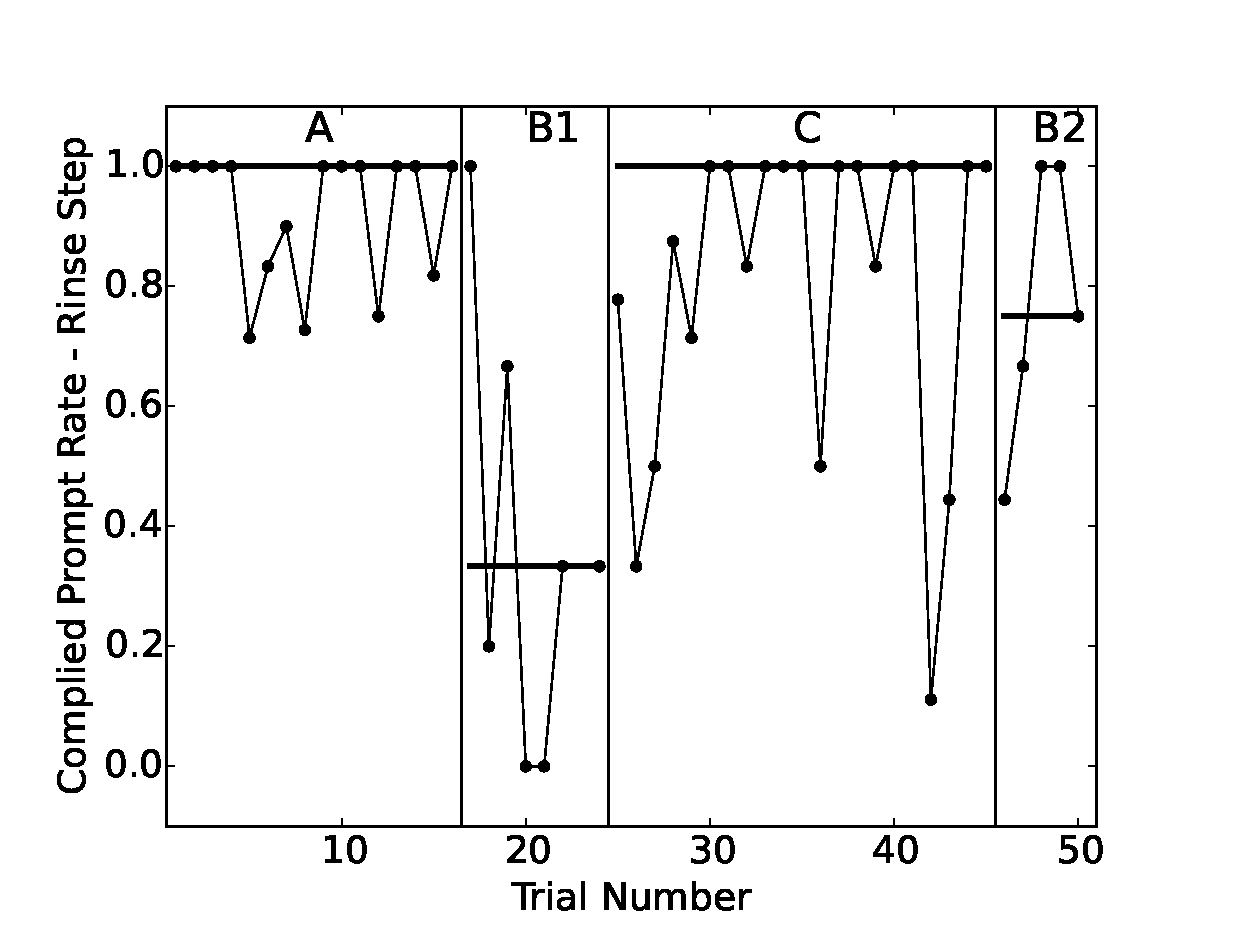
\includegraphics[width=0.6\textwidth]{./img/data_analysis/5CompliedPromptRate-RinseStep.eps}
	\caption{Rinse Step Complied Prompt Rate}
	\label{fig:5CompliedPromptRate-RinseStep}
\end{figure}

\subsubsection{Longest Duration of Rinse Step}
The Longest Duration of Rinse Step is plotted in Figure \ref{fig:8LongestDurationofRinsesec}, and has a median for Phase A of 7.15s, for Phase B1 of 2.87s, for Phase C of 5.36s, and for Phase B2 of 7.09s.  Although with high variance, we do see a distinct short duration during rinse step of Phase B1, and a retained improvement for Phase B2.
\begin{figure} [H]
	\centering
	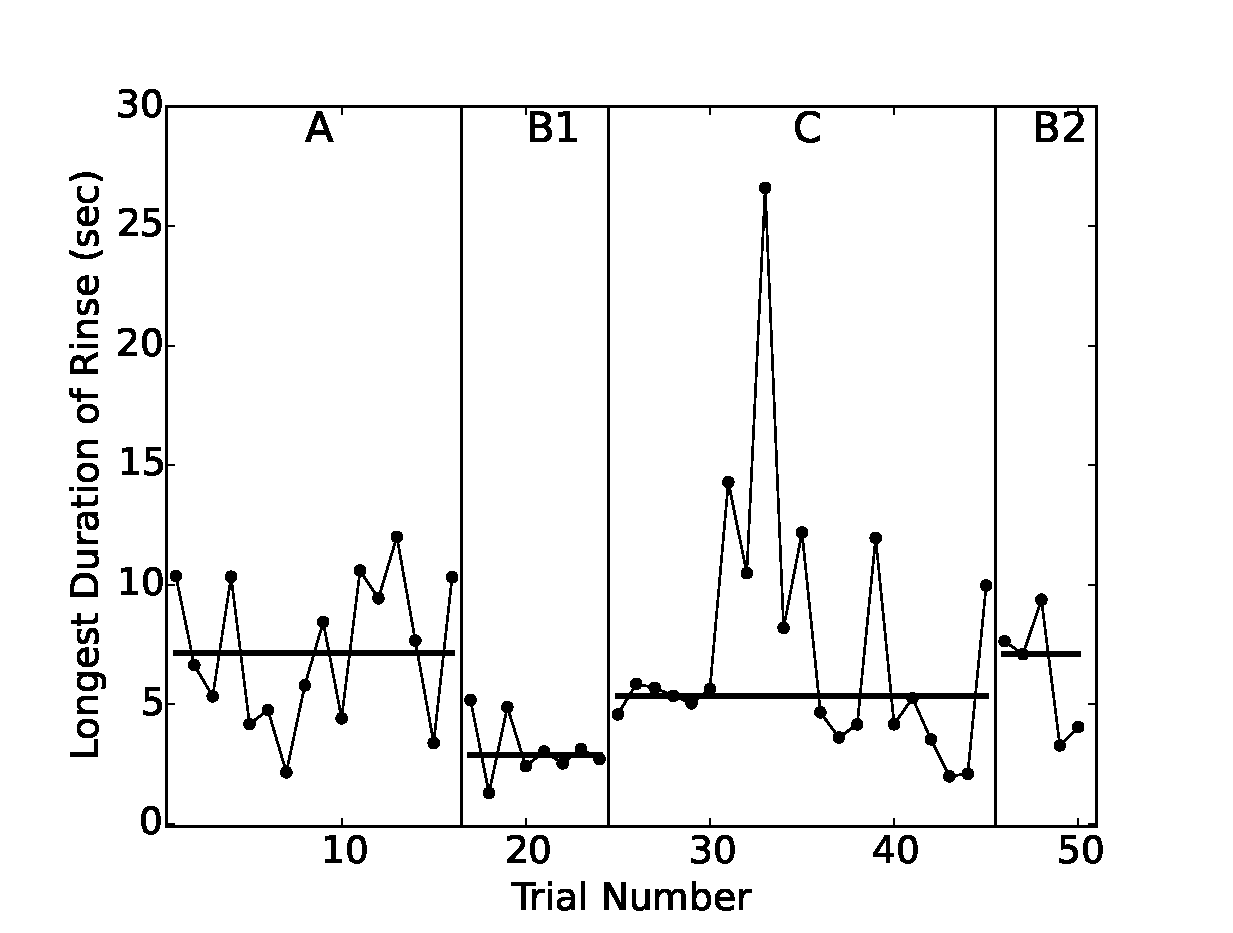
\includegraphics[width=0.6\textwidth]{./img/data_analysis/8LongestDurationofRinsesec.eps}
	\caption{Longest Duration of Rinse Step}
	\label{fig:8LongestDurationofRinsesec}
\end{figure}

\subsection{Qualitative Analysis and Results - Further}
After confirming our initial qualitative analysis results through quantitative measures on the child's improvements, we continue our qualitative analysis to answer what factors contributed to these improvements through parent researcher interview discussions and researcher self reflection.

\subsubsection{Causes of Child's Non-Compliances}
Between trials, the researcher (also taking the role of the robot operator) had frequent interview discussions with the mother (referred to as ``the parent'' in previous sections), and occasionally with the father, regarding reasons why the child had problems following the robot.

One major problem pointed out by both of the parents as well as the operator was the delay between each robot prompts.  This problem was particularly significant for our participant, who knew most of the steps of hand-washing, and only needed robot prompts to get started, to terminate the soap step, to rinse more, and to dry more.  Because of his familiarity with the hand-washing steps, he finished each step very quickly and was eager to move to the next step.  Thus a slight delay from the robot would result in the child not waiting for the robot prompts and proceeding on his own.  The mother first pointed this out in Phase B1, and the operator echoed her opinion, reflecting that it is hard to make the robot keep up with the child due to his pace and the robot delay.  The father also confirmed the opinion in Phase B2 that there should be less pause between prompts, especially for the rinse more prompts, as to prevent the child from moving onto the next step on his own.  Note that the father's opinion was based on the robot behavior after its improvements made to shorten its delays.

In addition, the parents proposed that unfamiliarity was a major cause of the child not following the robot prompts.  One possible cause for the child's noncompliance was his unfamiliarity with the robot and the washroom environment.  Both parents suggested that the child would be more relaxed and likely not rush each step if he was in a familiar environment, such as at home.  Furthermore, compliance would be greatly improved if the child and the robot built a relationship over time, the mother suggested, and if the robot was always there telling the child what to do, said the father.  To expand on his point, the father explained that the robot needed not to be an authoritative figure like his parents, but just needed to be a figure that the child is familiar in following instructions from, as exemplified by the child's tendency in following his younger brother's instructions.  The father further claimed that it was familiarity and routine, not trust.  The researcher noted that the environmental conditions between the parent trials and the robot trials were similar.  Thus, although being familiar with the environment would possibly improve compliance, the factor that contributed to the difference of child's compliance to the robot and to the parent can only be attributed to his unfamiliarity with the robot, not the environment.

Another possible cause for the child's noncompliance was fatigue due to repetitive consecutive hand-washing trials.  As pointed out by the father, during the robot trials, the child has been asked to wash his hands ten times in a roll with only five minutes of break between each time.  In addition, the robot prompted the rinse step for more than fifteen seconds each time, both of these may make the child unwilling to follow.  The father suggested to conduct each trial two to three hours apart, and prompt rinsing for only ten to fifteen seconds each time.  After further investigation, the researcher noted that the child's fatigue behavior was not specific to the robot, but also present during Phase A when the parent alone prompted the child.  The behavior manifested in the form of the child not willing to rinse more, but the exhibition of it was more subtle in the parent prompting case -- the child would comply to the parent's rinse more prompts, but he would only put his hands into the water for one second and quickly withdrew them and turned to look at the parent for approval to proceed to the next step, where as the child would openly refuse to rinse more in the robot's case.

Another possible cause for noncompliance was the child being confused of what was prompted or what was expected of him by the prompt.  However, there were evidences that the child understood most of the robot verbal prompts, if not all, because he was able to follow them at some point or another.  Thus, for the steps that the child did not follow, one can argue that it must have been due to a cause other than being generally confused of what was prompted.  The mother also confirmed that she thought the child was not confused by the robot prompts.  There were occasions when the child was confused, and they were when the parent pointed to the towel for the child to dry more after the child decided to leave the washroom.  The child would often mistook the parent's pointing gesture for rinse more, and started rinsing again instead of drying.  No such behavior occurred for robot prompts.


\subsubsection{Causes of Improvements of Child's Compliance}
There were three major factors identified by the researcher in potentially causing the improvements observed in the child's compliance to robot prompts: the first one was the improvements made to reduce robot prompt delays; the second was the child's gradual adjusting to the robot and to the routine of following its prompts; and the third was the effect of the trials in Phase C when the parent trained the child to follow the robot prompts.  Of course, there might be other important factors that happened during the time the child spent outside of the lab that were unaccounted for.

In regards to these three factors, the robot prompt delay improvement was seen as the least significant, since even after the improvement, we still could not achieve the responsiveness that the parent had during prompting.  The father also expressed he was not satisfied with the improved robot's responsiveness.   In addition, the effect on child's compliance by increasing the robot's responsiveness to the level of the parent was still unknown.

As to the other two factors, both involved the child learning to be guided by the robot, one from natural familiarization by himself and the other due to artificial training from the parent.  One may argue that, since the improvements mostly occurred after the second half of Phase C, it may suggest that the effect of artificial training from the parent was more dominant, since if it was the other way, then the child would have shown improvements earlier (e.g. after Phase B1 or during first half of Phase C).  However, this claim still lacks concrete evidence, and this question should be answered more rigorously by introducing a longer Phase B1 that is comparable to Phase C (in our study, we had one week for Phase B1, but two weeks for Phase C) so that the learning effects of the two phases can be compared.


\subsubsection{Post-Intervention Survey for Parent}
The post-intervention survey results are presented in Table \ref{tab:PostInterventionSurveyData}.  We see that the parent was happy with all aspects of the robot as a prompting agent, but did not see it to be as good as herself yet in delivering effective prompting.

In addition, the suggestions the parent made regarding the robot and the experiment are reported:  The robot can improve its pointing better so that the child sees exactly which object he needs to interact with.  This can be done by having more fingers on the robot's hands, or by attaching a light source (e.g. laser pointer or mini-projector) that the robot can use to highlight physical objects at the sink.  The robot would be more visible if it is bigger or placed at eye level of the child.  It would be ideal if the robot is mobile, and can prompt other activities of daily living besides hand-washing.  Lastly, attaching permanent cameras in the washroom is not okay, since the child is not the only one using the washroom.  Thus, having a mobile robot that follows the child would be a better solution.



\begin{table}[H]
	\centering
	\begin{tabular}{ | p{12cm} | l | }
		\hline
		\textbf{Survey Question}	&	\textbf{Parent's Answer}	\\	\hline	\hline		
		Hand-washing steps break down was appropriate	&	Strongly Agree	\\	\hline
		My child understood the verbal prompts	&	Agree	\\	\hline
		Robot's verbal prompts were appropriate	&	Strongly Agree	\\	\hline
		The prompt wordings were similar to mine	&	Strongly Agree	\\	\hline
		The prompt voice and tone were appropriate	&	Strongly Agree	\\	\hline
		The prompt wordings were easy to understand	&	Strongly Agree \\	\hline
		My child understood the gesture prompts	&	Strongly Agree	\\	\hline
		The gesture prompts were appropriate	&	Strongly Agree	\\	\hline
		The gesture prompts were easy to understand	&	Agree	\\	\hline
		The physical appearance of robot is aesthetically pleasing	&	Agree	\\	\hline
		The attention grabber gestures were appropriate	&	Strongly Agree	\\	\hline
		The verbal rewards were appropriate	&	Strongly Agree	\\	\hline
		The reward gestures were appropriate	&	Strongly Agree	\\	\hline
		The robot was effective in assisting my child through hand-washing	&	Strongly Agree	\\	\hline
		The robot motivated my child to wash hands	&	Strongly Agree	\\	\hline
		The robot was fun for my child to use	&	Strongly Agree	\\	\hline
		My child was confused by the robot	&	Disagree	\\	\hline
		I like the idea of a robot prompting my child	&	Strongly Agree	\\	\hline
		The robot is able to provide guidance as well as I can or better	&	Neither Agree or Disagree	\\	\hline
		I would want to own a robot like this one	&	Strongly Agree	\\	\hline
	\end{tabular}
	\caption{The Post-Intervention Survey Data}
	\label{tab:PostInterventionSurveyData}
\end{table}

